\documentclass[10pt]{extarticle}
\title{}
\author{}
\date{}
\usepackage[shortlabels]{enumitem}


%paper setup
\usepackage{geometry}
\geometry{letterpaper, portrait, margin=1in}
\usepackage{fancyhdr}
% sans serif font:
\usepackage{cmbright}
%symbols
\usepackage{amsmath}
\usepackage{bigints}
\usepackage{amssymb}
\usepackage{amsthm}
\usepackage{mathtools}
\usepackage{bbm}
\usepackage[hidelinks]{hyperref}
\usepackage{gensymb}
\usepackage{multirow,array}
\usepackage{multicol}

\newtheorem*{remark}{Remark}
\usepackage[T1]{fontenc}
\usepackage[utf8]{inputenc}

%chemistry stuff
%\usepackage[version=4]{mhchem}
%\usepackage{chemfig}

%plotting
\usepackage{pgfplots}
\usepackage{tikz}
\tikzset{middleweight/.style={pos = 0.5}}
%\tikzset{weight/.style={pos = 0.5, fill = white}}
%\tikzset{lateweight/.style={pos = 0.75, fill = white}}
%\tikzset{earlyweight/.style={pos = 0.25, fill=white}}

%\usepackage{natbib}

%graphics stuff
\usepackage{graphicx}
\graphicspath{ {./images/} }
\usepackage[style=numeric, backend=biber]{biblatex} % Use the numeric style for Vancouver
\addbibresource{the_bibliography.bib}
%code stuff
%when using minted, make sure to add the -shell-escape flag
%you can use lstlisting if you don't want to use minted
%\usepackage{minted}
%\usemintedstyle{pastie}
%\newminted[javacode]{java}{frame=lines,framesep=2mm,linenos=true,fontsize=\footnotesize,tabsize=3,autogobble,}
%\newminted[cppcode]{cpp}{frame=lines,framesep=2mm,linenos=true,fontsize=\footnotesize,tabsize=3,autogobble,}

%\usepackage{listings}
%\usepackage{color}
%\definecolor{dkgreen}{rgb}{0,0.6,0}
%\definecolor{gray}{rgb}{0.5,0.5,0.5}
%\definecolor{mauve}{rgb}{0.58,0,0.82}
%
%\lstset{frame=tb,
%	language=Java,
%	aboveskip=3mm,
%	belowskip=3mm,
%	showstringspaces=false,
%	columns=flexible,
%	basicstyle={\small\ttfamily},
%	numbers=none,
%	numberstyle=\tiny\color{gray},
%	keywordstyle=\color{blue},
%	commentstyle=\color{dkgreen},
%	stringstyle=\color{mauve},
%	breaklines=true,
%	breakatwhitespace=true,
%	tabsize=3
%}
% text + color boxes
\renewcommand{\mathbf}[1]{\mathbbm{#1}}
\usepackage[most]{tcolorbox}
\tcbuselibrary{breakable}
\tcbuselibrary{skins}
\newtcolorbox{problem}[1]{colback=white,enhanced,title={\small #1},
          attach boxed title to top center=
{yshift=-\tcboxedtitleheight/2},
boxed title style={size=small,colback=black!60!white}, sharp corners, breakable}
%including PDFs
%\usepackage{pdfpages}
\setlength{\parindent}{0pt}
\usepackage{cancel}
\pagestyle{fancy}
\fancyhf{}
\rhead{Avinash Iyer}
\lhead{Math 212: Homework 10}
\newcommand{\card}{\text{card}}
\newcommand{\ran}{\text{ran}}
\newcommand{\N}{\mathbbm{N}}
\newcommand{\Q}{\mathbbm{Q}}
\newcommand{\Z}{\mathbbm{Z}}
\newcommand{\R}{\mathbbm{R}}
\begin{document}
  \begin{problem}{18.4}
    \begin{description}[font=\normalfont]
      \item[2:] $f(x,y) = x^2y$
      \item[6:] $f(x,y) = x^2y^3 + xy$
      \item[10:] There is no function that serves this purpose.
      \item[12:]
        \begin{align*}
          \oint_{C}\vec{F} \cdot d\vec{r} &= \int_{R} \left(\frac{\partial F_2}{\partial x} - \frac{\partial F_1}{\partial y}\right)~dx~dy\\
                                          &= \int_{0}^{1}\int_{0}^{1} -x~dx~dy\\
                                          &= \frac{1}{2}
        \end{align*}
      \item[14:]
        \begin{align*}
          \oint_{C}\vec{F} \cdot d\vec{r} &= \int_{R} \left(\frac{\partial F_2}{\partial x} - \frac{\partial F_1}{\partial y}\right)~dx~dy\\
                                          &= \int_{R} \left(x-3\right)~dx~dy\\
                                          &= \int_{0}^{2\pi}\int_{0}^{1}(r\cos\theta - 3)r~dr~d\theta\\
                                          &= -3\pi
        \end{align*}
      \item[24:]
        \begin{align*}
          \oint_{C}\vec{F} \cdot d\vec{r} &= \int_{0}^{1}\int_{x^3}^{x^2} \left(\frac{\partial F_2}{\partial x} - \frac{\partial F_1}{\partial y}\right)~dy~dx\\
                                          &= \int_{0}^{1}\int_{x^3}^{x^2}\left(-y\right)~dy~dx\\
                                          &= \frac{1}{2}\int_{0}^{1} x^6-x^4~dx\\
                                          &= \frac{1}{35}
        \end{align*}
      \item[28:]
        \begin{enumerate}[(a)]
          \item $\int_{C} \vec{F}\cdot d\vec{r} = f(2,4) - f(0,0) = 4e^{4}$
          \item $\int_{C} \vec{G}\cdot d\vec{r} = 4$
        \end{enumerate}
      \item[34:]
        \begin{align*}
          \int_{C} \vec{F} \cdot d\vec{r} &= \int_{R} 1~dx~dy
        \end{align*}
    \end{description}
  \end{problem}
  \begin{problem}{19.1}
    \begin{description}[font=\normalfont]
      \item[2:] 
        \begin{align*}
          \vec{A} &= \begin{pmatrix}0\\0\\25\pi\end{pmatrix}
        \end{align*}
      \item[4:]
        \begin{align*}
          \vec{A} &= \begin{pmatrix}0\\15\\0\end{pmatrix}
        \end{align*}
      \item[8:]
        \begin{enumerate}[(a)]
          \item Negative
          \item Positive
          \item Negative
          \item Negative
          \item Zero
        \end{enumerate}
      \item[12:]
        \begin{enumerate}[(a)]
          \item $-32\pi$
          \item $32\pi$
        \end{enumerate}
      \item[16:]
        \begin{align*}
          \vec{A} &= \begin{vmatrix}\hat{i} & \hat{j} & \hat{k} \\ 0 & 2 & 0 \\ -2 & 0 & 3\end{vmatrix}\\
                  &= \begin{pmatrix}6\\0\\4\end{pmatrix}\\
          \vec{v} \cdot \vec{A} &= -6
        \end{align*}
      \item[20:]
        \begin{align*}
          \vec{n} &= \begin{vmatrix}\hat{i} & \hat{j} & \hat{k} \\ -1 & 1 & 0 \\ 0 & -1 & 1\end{vmatrix}\\
                  &= \begin{pmatrix}1\\1\\1\end{pmatrix}\\
          \hat{n} &= \frac{1}{\sqrt{3}}\vec{n}\\
          \vec{A} &= \frac{\sqrt{3}}{2}\frac{1}{\sqrt{3}}\vec{n}\\
                  &= \begin{pmatrix}1/2\\1/2\\1/2\end{pmatrix}\\
          \vec{v} \cdot \vec{A} &= \frac{3}{2}
        \end{align*}
      \item[26:]
        \begin{align*}
          \int_{S}\vec{H}\cdot d\vec{A} &= 3
        \end{align*}
      \item[30:]
        \begin{align*}
          \int_{S} \vec{F} \cdot d\vec{A} &= 45\pi
        \end{align*}
      \item[40:]
        \begin{align*}
          \int_{S} \vec{F} \cdot d\vec{A} &= 28\pi
        \end{align*}
      \item[50:]
        \begin{align*}
          \int_{S} \vec{F} \cdot d\vec{A} &= \int_{0}^{2}\int_{0}^{3}\left(2z + 4\right)~dz~dy\\
                                          &= 42
        \end{align*}
    \end{description}
  \end{problem}
  \begin{problem}{19.2}
    \begin{description}[font=\normalfont]
      \item[2:]
        \begin{align*}
          \vec{A} &= \begin{pmatrix}-8\\-7\\1\end{pmatrix}
        \end{align*}
      \item[4:]
        \begin{align*}
          \vec{A} &= \begin{pmatrix}-y\\-x-2y\\1\end{pmatrix}
        \end{align*}
      \item[6:]
        \begin{align*}
          \int_{S}\vec{F}\cdot d\vec{A} &= \int_{0}^{8}\int_{0}^{4} \left((-4)(50-4x+10y) + 10x +y\right)~dx~dy
        \end{align*}
      \item[12:]
        \begin{align*}
          \int_{S}\vec{F} \cdot d\vec{A} &= \int_{0}^{1}\int_{-1}^{1}(2x + y + 2)~dx~dy\\
                                         &= \frac{5}{2}
        \end{align*}
      \item[16:] 
      \item[18:] 
      \item[20:]
      \item[22:]
        \begin{align*}
          \int_{S} \vec{F} \cdot d\vec{A} &= \int_{0}^{2\pi}\int_{0}^{\pi}\left(25\sin\phi(\sin^2\phi\cos^2\theta + 2\sin^2\phi\sin^2\theta + 3\cos^2\theta)\right)~d\phi~d\theta
        \end{align*}
      \item[24:]
        \begin{align*}
          \int_{S} \vec{F} \cdot d\vec{A} &= \int_{0}^{\pi}\int_{0}^{\pi/2}9\sin\phi\cos\phi e^{\cos\theta\sin\phi}~d\phi~d\theta
        \end{align*}
    \end{description}
  \end{problem}
  \begin{problem}{19.3}
    \begin{description}[font=\normalfont]
      \item[2:] Scalar:
        \begin{align*}
          \nabla \cdot \begin{pmatrix}2\sin(xy) + \tan(z) \\ \tan(y) \\ e^{x^2 + y^2}\end{pmatrix} &= 2y\cos(xy) + \sec^2(y)
        \end{align*}
      \item[4:]
        \begin{align*}
          \nabla \cdot \vec{F} &= 0
        \end{align*}
      \item[6:]
        \begin{align*}
          \nabla \cdot \vec{F} &= -1
        \end{align*}
      \item[24:]
        \begin{align*}
          \nabla \cdot \nabla F &= \begin{pmatrix}\frac{\partial}{\partial x}\\\frac{\partial}{\partial y}\end{pmatrix} \cdot \begin{pmatrix}ay + 2axy\\ax + ax^2 + 3y^2\end{pmatrix}\\
                                &= 2ay + 6y\\
          a &= \boxed{-3}
        \end{align*}
      \item[28:]
        \begin{align*}
          \nabla \cdot \vec{F} &= 1
        \end{align*}
        Viewed facing the $yz$ plane, we can see the following field, which indicates that the vector field does have zero divergence.
        \begin{center}
          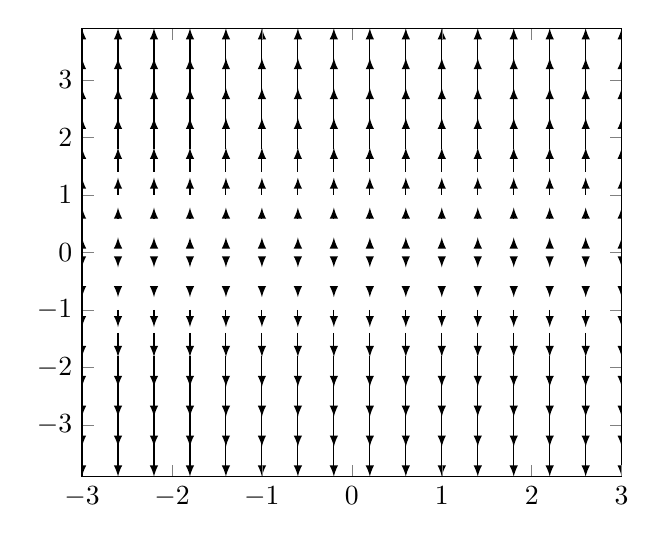
\begin{tikzpicture}
            \begin{axis}[
                view = {0}{90},
                domain= -3:3,
                y domain= -3:3,
                xtick={-3,...,3},
                ytick={-3,...,3}
              ]
              \addplot3[black,quiver={u=0,v=y,scale arrows=0.3},samples=16, -latex](x,y,0);
            \end{axis}
          \end{tikzpicture}
        \end{center}
      \item[38:]
    \end{description}
  \end{problem}
\end{document}
